%%%%%%%%%%%%%%%%%%%%%%%%%%%%%%%%%%%%%%%%%%%%%%%%%%%%%%%%%%%%%%%%%%%%%%%%%%%%%%%%
% Template for USENIX papers.
%
% History:
%
% - TEMPLATE for Usenix papers, specifically to meet requirements of
%   USENIX '05. originally a template for producing IEEE-format
%   articles using LaTeX. written by Matthew Ward, CS Department,
%   Worcester Polytechnic Institute. adapted by David Beazley for his
%   excellent SWIG paper in Proceedings, Tcl 96. turned into a
%   smartass generic template by De Clarke, with thanks to both the
%   above pioneers. Use at your own risk. Complaints to /dev/null.
%   Make it two column with no page numbering, default is 10 point.
%
% - Munged by Fred Douglis <douglis@research.att.com> 10/97 to
%   separate the .sty file from the LaTeX source template, so that
%   people can more easily include the .sty file into an existing
%   document. Also changed to more closely follow the style guidelines
%   as represented by the Word sample file.
%
% - Note that since 2010, USENIX does not require endnotes. If you
%   want foot of page notes, don't include the endnotes package in the
%   usepackage command, below.
% - This version uses the latex2e styles, not the very ancient 2.09
%   stuff.
%
% - Updated July 2018: Text block size changed from 6.5" to 7"
%
% - Updated Dec 2018 for ATC'19:
%
%   * Revised text to pass HotCRP's auto-formatting check, with
%     hotcrp.settings.submission_form.body_font_size=10pt, and
%     hotcrp.settings.submission_form.line_height=12pt
%
%   * Switched from \endnote-s to \footnote-s to match Usenix's policy.
%
%   * \section* => \begin{abstract} ... \end{abstract}
%
%   * Make template self-contained in terms of bibtex entires, to allow
%     this file to be compiled. (And changing refs style to 'plain'.)
%
%   * Make template self-contained in terms of figures, to
%     allow this file to be compiled. 
%
%   * Added packages for hyperref, embedding fonts, and improving
%     appearance.
%   
%   * Removed outdated text.
%
%%%%%%%%%%%%%%%%%%%%%%%%%%%%%%%%%%%%%%%%%%%%%%%%%%%%%%%%%%%%%%%%%%%%%%%%%%%%%%%%

\documentclass[letterpaper,twocolumn,10pt]{article}
\usepackage{usenix2020}

% to be able to draw some self-contained figs
\usepackage{tikz}
\usepackage{amsmath}

% inlined bib file
\usepackage{filecontents}

\usepackage{graphicx}
\graphicspath{{\downloads }}

%-------------------------------------------------------------------------------
\begin{filecontents}{\jobname.bib}
%-------------------------------------------------------------------------------
@Book{arpachiDusseau18:osbook,
  author =       {Arpaci-Dusseau, Remzi H. and Arpaci-Dusseau Andrea C.},
  title =        {Operating Systems: Three Easy Pieces},
  publisher =    {Arpaci-Dusseau Books, LLC},
  year =         2015,
  edition =      {1.00},
  note =         {\url{http://pages.cs.wisc.edu/~remzi/OSTEP/}}
}
@InProceedings{waldspurger02,
  author =       {Waldspurger, Carl A.},
  title =        {Memory resource management in {VMware ESX} server},
  booktitle =    {USENIX Symposium on Operating System Design and
                  Implementation (OSDI)},
  year =         2002,
  pages =        {181--194},
  note =         {\url{https://www.usenix.org/legacy/event/osdi02/tech/waldspurger/waldspurger.pdf}}}
\end{filecontents}

%-------------------------------------------------------------------------------
\begin{document}
%-------------------------------------------------------------------------------
% make title bold and 14 pt font (Latex default is non-bold, 16 pt)
\title{\bf CS 131: Final Project Report \\ 
		\large Implementing a proxy herd with asyncio}
\author{Carson Kim - Winter 2021}
\maketitle

%-------------------------------------------------------------------------------
\section{Abstract}
%-------------------------------------------------------------------------------

This report will mainly discuss the pros of the \verb +asyncio+ library and its utility in an application server herd designed for rapidly-evolving data. I will discuss compatibility, ease of use, performance implications, and whether or not it is important to use the latest features offered by Python 3.9 or later. Moreover, the paper will discuss language-specific issues relating to Python - including type-checking, memory management, and multithreading. Lastly, I will be comparing the  \verb +asyncio+ library with the Node.js approach. 


%-------------------------------------------------------------------------------
\section{Introduction}
%-------------------------------------------------------------------------------
\verb +asyncio+ is Python's flagship library used for several foundational frameworks that allows concurrent, controlled execution over Python coroutines. In addition, it provides several high-level APIs for performing network input and output between server and client as well as the synchronization of concurrent code. These APIs proved to be rather intuitive when implementing a server herd for a Wikimedia-style service, and the rest of the paper will explore why I can give it a strong recommendation for such purposes. 
%-------------------------------------------------------------------------------

%-------------------------------------------------------------------------------
\section{Ease of Use}
%-------------------------------------------------------------------------------
The  \verb +asyncio+ library has intuitive, clean syntax. The typical way to declare coroutines is through the \verb +await+ and \verb +async+ keywords. These keywords appeared mainly in my server class, where the majority of the work was being done. This included declaring functions that handle client input as well as propagate messages as async functions, and the coroutines within them were declared with the \verb +await+ keyword. 

According to the \verb +asyncio+ Python documentation, these coroutines are known as awaitables and can be accepted by the \verb +asyncio.run()+ function. This main function is responsible for managing the event loop and is the main point of entry for \verb +asyncio+ programs. I found this to work quite well with my program, as I included a function that "runs forever" and is where all important coroutines are executed. 


%-------------------------------------------------------------------------------
\section{Performance Implications / Compatibility}
%-------------------------------------------------------------------------------
 \verb +asyncio+ makes running concurrent, asynchronous code quite easy. It confers more power to the programmer in how they decide to control tasks / functions, and has stronger scheduling than the normal Python interpreter. Without \verb +asyncio+, the Python interpreter could bleed resources by interrupting trivial tasks to switch to other threads. 

\verb +asyncio+ seems to be quite compatible with the objectives of the server herd. Since we are required to make https requests, I did have to import the \verb +aiohttp+ module. This module is dependent on the \verb +asyncio+ library but makes it quite easy to run an event loop that declares a \verb +ClientSession()+ object that returns a response object that we can print and or manipulate. For these reasons,  \verb +asyncio+ seems to achieve optimized, desired behavior.

%-------------------------------------------------------------------------------
\section{Problems Encountered}
%-------------------------------------------------------------------------------
The main difficulties of this project arose when propagating AT messages to other servers. First, there was the question of how this would be achieved. I decided that including a global dictionary that contained all of the server relationships could be useful here. Each server has a list of servers it can speak to, so naturally we should be able to traverse through this list and make sure the message is sent to each one. Of course, the function that handled this task was declared as asynchronous. 

The other challenge was deciding when to propagate messages. There must be a condition under which servers do not propagate further, or else duplicate messages would be constantly bothering their server neighbors, resulting in an infinite loop. I did encounter this issue, and it ended up flooding my log files with repeated instances of the same request / action. These files ended up growing enormously large and eating up nearly all of my available disk space on my seas.net account. This spawned a number of problems, but it certainly taught me to be more careful in writing smarter, loop-free code. 

%-------------------------------------------------------------------------------
\section{Overall Design}
%-------------------------------------------------------------------------------
The overall design of my program relied on several \verb +async def+ methods within my server class that would handle client input, retrieve the JSON response via the Google API search request, and propagate the messages to its nearby servers. The non-asynchronous functions were responsible for parsing and validating the arguments sent by the client. Of course, the server class also contains private variables that store the most recent coordinate info for every client as well as its timestamp. This is to ensure that servers always receive the most up-to-date information so they can handle WHATSAT requests properly. 

Logging was done via Python's \verb +logging+ module. As required by the project spec, the log keeps track of all messages received by the server as well as its responses. The log also records any attempted connections to neighboring servers and alerts the user when an attempt fails. Figures 1 and 2 show brief snippets of Riley and Bernard's server logs when prompted with some simple requests mentioned in the spec. I intentionally closed connections for Juzang and Bernard to demonstrate that the other servers record any known outages yet still propagate to their other neighbors if possible.

\begin{figure}

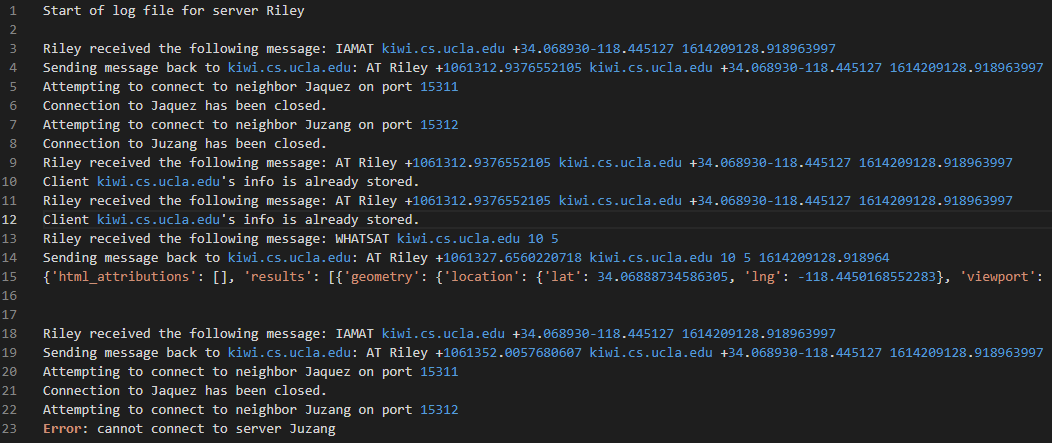
\includegraphics[scale=.2]{rileylog.PNG}
\caption{\label{fig:vectors} Logging info stored for server Riley}
\end{figure}


\begin{figure}

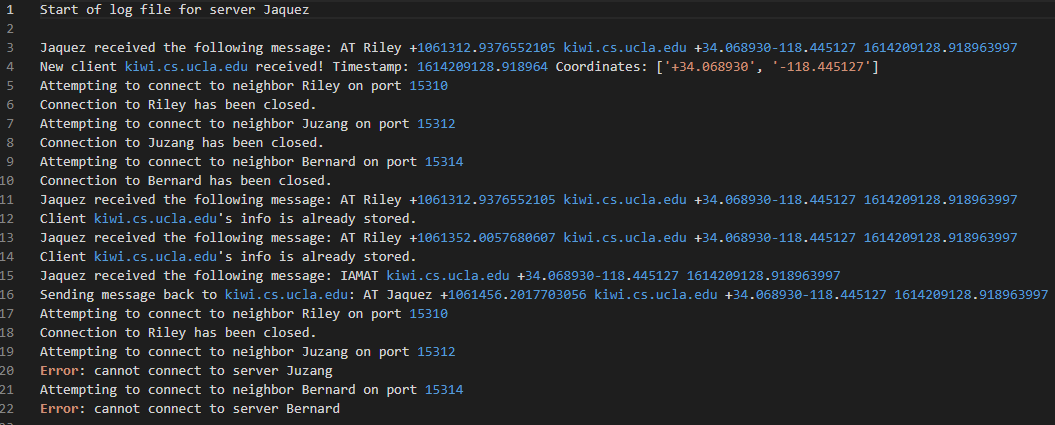
\includegraphics[scale=.2]{jaquezlog.PNG}
\caption{\label{fig:vectors} Logging info stored for server Jaquez} 
\end{figure}



%-------------------------------------------------------------------------------
\section{Python vs. Java}
%-------------------------------------------------------------------------------
This section will briefly discuss the advantages / disadvantages of a Python-based approach over Java in the implementation of this project. 

\subsection{Type Checking}
Python's type checking system proved to be quite beneficial when working on this project, as it saved a lot of unnecessary programming hassle. Since Python is a dynamically typed language, there was no need to declare \verb +asyncio+ objects or coroutines as a certain type. A Java approach would likely have resulted in more verbose code that would have to accommodate to its static type checking requirements. I did not run into any runtime errors that resulted from type misinterpretations, and Python made it easy to write fast, fluid code that included a module with which I was completely unfamiliar.

\subsection{Memory Management}

Python utilizes an approach to garbage collection known as reference counting. Oftentimes, reference counting can be slower than Java's approach which involves identifying dead areas of code. In addition, Java's memory manager only allocates memory to objects and its garbage collector frees null pointers. It seems that since that Python's reliance on references to clean up objects could lead to worsened performance than Java, which has a much more robust and "smarter" way of determining dead code. 


\subsection{Multithreading}

Since Python is an interpreted language, it naturally has an unconventional way of thread monitoring compared to its compile-time counterparts. The CPython interpreter doesn't even support multithreading, and the global interpreter lock is only responsible for isolated thread execution without actually providing any lock mechanisms to guarantee there aren't data races. Java offers keywords such as \verb +synchronized+ and \verb +volatile+ to help deal with shared resources in a program. The Java Memory Model's allowance of multithreading could potentially lead to increased risks in data races. For this project, it seems like Python should suffice as only one thread is required to run anyway. 



%-------------------------------------------------------------------------------
\section{Asyncio vs. Node.js}
%-------------------------------------------------------------------------------

Node.js relies on callbacks to accomplish asynchronous behavior, but it appears as if it is quite similar to \verb +asyncio+ in their approach and design. Both can utilize the aforementioned awaitables that take in coroutines, and both run a main event loop. Such asynchronous functions are key to both  \verb +asyncio+ and Node.js. Node.js can require some more advanced control flow to handle more complicated asynchronous tasks, but overall is rather competitive when compared to an  \verb +asyncio+ approach. 




\section{Reliance on Latest Python Features}

The release of Python 3.9 doesn't seem like it would disrupt a programmer's use of old features. According to recent documentation, most updates involve updates to event loop handlers. The \verb +asyncio.run()+ function would be the only major impact, as it now relies on coroutines to accomplish desired behavior. These coroutines, as mentioned earlier in the report, are declared with the async def keywords. There are other options available for implementing event loops, however. Namely, the \verb +new_event_loop()+ function which creates a new event loop that can do most of the work.  


%-------------------------------------------------------------------------------
\section{Conclusion}
%-------------------------------------------------------------------------------
Overall, this project provided useful insight into the advantages of Python's \verb +asyncio+ networking library. Due to its intuitive methods of running event loops and handling coroutines, I think the module is a strong candidate for replacing the Wikimedia platform for my application. It works seamlessly with not only TCP requests but also HTTP requests, with great help from the \verb +aiohttp+ library. Python's slick type checking system also allows for fluid, cleaner code when working with this particular module. Through this experience, I can guarantee that any application developed with \verb +asyncio+ functions is maintainable and reliable. 


%-------------------------------------------------------------------------------
\ 
%-------------------------------------------------------------------------------
\section{References}

\url {https://docs.python.org/3/whatsnew/3.9.html#asyncio} \\
\url {https://docs.aiohttp.org/en/stable/client_quickstart.html}\\
\url {https://eng.paxos.com/python-3s-killer-feature-asyncio}\\
\url {https://towardsdatascience.com/a-better-way-for-asynchronous-programming-asyncio-over-multi-threading-3457d82b3295}\\
\url {https://medium.com/@interfacer/intro-to-async-concurrency-in-python-and-node-js-69315b1e3e36}\\











%%%%%%%%%%%%%%%%%%%%%%%%%%%%%%%%%%%%%%%%%%%%%%%%%%%%%%%%%%%%%%%%%%%%%%%%%%%%%%%%
\end{document}
%%%%%%%%%%%%%%%%%%%%%%%%%%%%%%%%%%%%%%%%%%%%%%%%%%%%%%%%%%%%%%%%%%%%%%%%%%%%%%%%

%%  LocalWords:  endnotes includegraphics fread ptr nobj noindent
%%  LocalWords:  pdflatex acks
